% This is LLNCS.DEM the demonstration file of
% the LaTeX macro package from Springer-Verlag
% for Lecture Notes in Computer Science,
% version 2.4 for LaTeX2e as of 16. April 2010
%
\documentclass{llncs}
%
\usepackage{makeidx}  % allows for indexgeneration
\usepackage{amsmath}
\usepackage{amssymb}
\usepackage{graphicx}
\usepackage{tikz}

%
\begin{document}
%
\mainmatter              % start of the contributions
%
\title{An Executable Formal Semantics For A Functional Actor Language}
%
\author{Xiaohong Chen, Lucas Pe\~{n}a}
%
\institute{University of Illinois at Urbana-Champaign, \\
\email{\{xc3, lpena7\}@illinios.edu}}

\maketitle              % typeset the title of the contribution

\begin{abstract}
A simple reference actor language has been proposed in~\cite{}, serving as a
sound mathematical calculus foundation for various actor languages used in
distributed applications that involves concurrency. Even though the authors
of~\cite{} provided in the paper an operational semantics of the actor language,
an executable implementation was not given. In this project, we will give the
reference actor language an implementation that by construction conforms to its
formal operational semantics using the K framework~\cite{}, a rule-based
semantic framework. We will show that our executable formal semantics are
capable of executing some meaningful actor systems examples. We hope our
executable formal semantics can be served as a starting point for future work in
developing automatic equivalence provers using the K framework.
\end{abstract}
%
\section{Introduction}
The K framework~\cite{} is a framework for defining executable operational
semantics of a programming language. K is based on rewriting logic, organizing
the state of a program into cells and rewriting the particular parts of the
configuration. K also has access the entire computation at any particular
time. These features and more allow for difficult language constructs to be
designed with ease in K. On top of that, K provides backend tooling for
additional features based on the semantics of a programming language, such as a
semantic debugger and a full formal verifier. See Figure~\ref{fig:k-tools} for a
complete view of the tools one gets from K based off an operational semantics.

In the rest of the paper we discuss related work, then the actor semantics in
some detail, including the configuration, the syntax and how we handle reduction
contexts in K, the semantics, and an in-depth example. We then conclude and
discuss future work.

\section{Related Work}

\begin{figure}
          \centering
          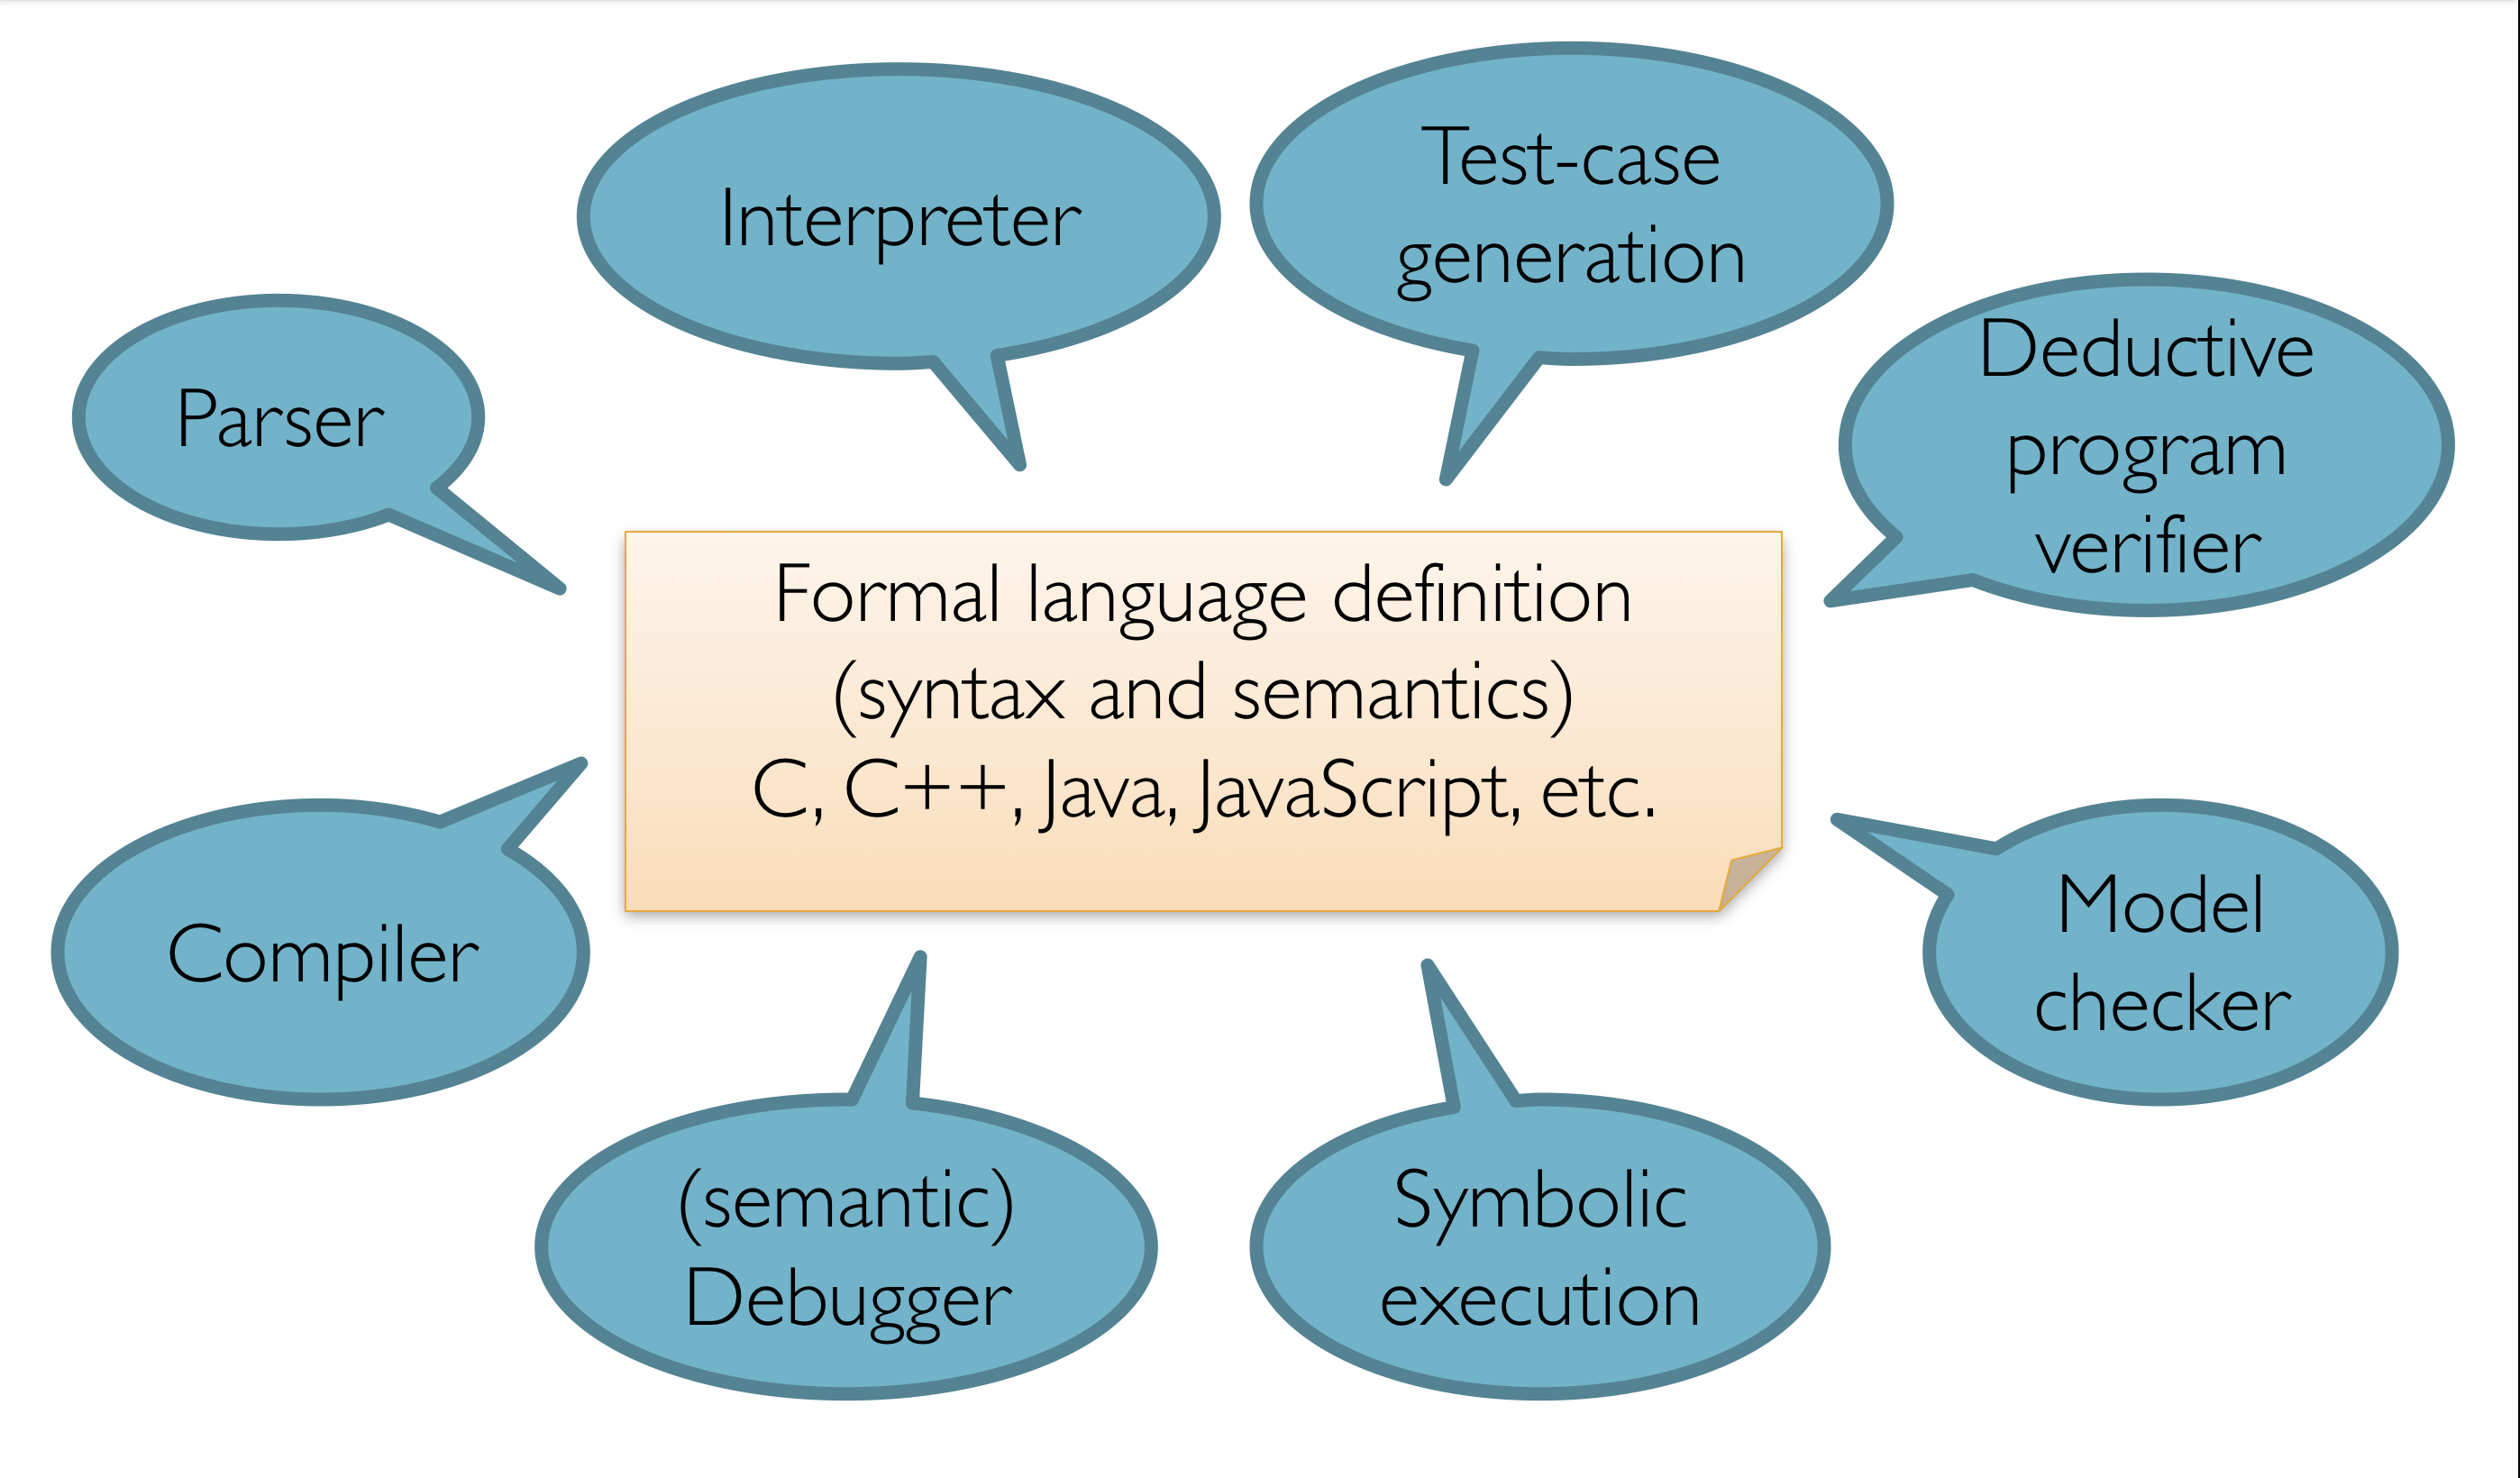
\includegraphics[scale=0.13]{../k-overview.png}
	  \caption{Backend tools K provides from just an operational
            semantics. Some tools such as a semantics-based compiler and
            test-case generation are in progress.}
          \label{fig:k-tools}
\end{figure}
To demonstrate the power of K, languages as complex as C, Java, and JavaScript
have been fully defined using the K framework~\cite{c,java,jscript}. On top of that, in
all of these languages and more, nontrivial programs have been formally verified
using K's prover, such as proofs involving AVL trees and red-black trees. We
would like to add an actor-based language to the growing list of languages
defined in K, so we can take advantage of K's formal verification engine and
more.

Semantics of actor-based languages have been defined on paper, for example
in~\cite{}. Additionally, there are many implementations of actor-based systems,
including Erlang~\cite{}, Akka~\cite{}, Scheme~\cite{}, and much more. However,
there is currently no formally defined \textit{executable} operational semantics
of an actor-based language. In K, there was previous work done to define the
semantics of Orc, a concurrent programming language~\cite{}, though that work is
incomplete.

In this paper, we aim to define the semantics of the actor language proposed
in~\cite{}.  We choose this language as the semantics are clearly defined in the
paper, and it is one of the more simple actor frameworks. Defining this language
in K will give assurance to the correctness of the language - as K is executable
this can be tested much easier than defining a language on paper. It will also
provide more assurance on K's language-defining ability, as well as open up to
formal analysis using the tools seen in Figure~\ref{fig:k-tools}.

\section{The Actor Language in K}
In this section, we describe in detail some important features of the actor
language from~\cite{}. We cover some important features from K and how they were
used to define key concepts of the actor language.

\subsection{Configuration}
All languages in K use a configuration to specify the current state of a
program. For simple languages like the lambda calculus or a simple \texttt{IMP}
language, there may only be one cell to hold the current computation (the
\texttt{k} cell) and perhaps another \texttt{env} cell for the current
environment. For the actor language, we have the following configuration:
\begin{verbatim}
configuration 
  <T>
    <actors>
      <actor multiplicity="*">     // a multiset of actors
        <k> exec($PGM:Exp) </k>    // actor state
        <id> initactor </id>       // actor id
      </actor>
    </actors>
    <messages>
      <message  multiplicity="*">  // a multiset of messages
        .K
      </message>
    </messages>
    <definedaddr>                  // list of defined actors'
      ListItem(initactor)          // addresses
    </definedaddr>
  </T>
\end{verbatim}
In addition to defining the state of a program, the configuration is also used
to define the initial state of a program. Initially, we only have one actor,
with the unique identifier \texttt{initactor}. It also contains the program in
the \texttt{exec} state ready to be executed. The variable \texttt{\$PGM} comes
from an external file. The notation \texttt{multiplicity=*} is used to specify
that there can be any number of \texttt{actor} cells and \texttt{message} cells
as a multiset of actors and messages respectively. Initially there are no
messages, represented using K's builtin \texttt{.K}. Finally, the
\texttt{definedaddr} cell is used to keep track of addresses of defined
actors. We need to keep track of this for the side condition of some semantic
rules (see Section~\ref{sec:semantics}).

For our K definition, we only define a single actor system, so there are no
external actors or receptionists. To add these one can simply add these as
additional cells in the configuration, initialized to the empty list.

\subsection{Syntax and Reduction Contexts}
Syntax for constructs in K is specified using BNF notation. For example, we
specify values (where reduction can no longer happen) as
\begin{verbatim}
  syntax Val  ::= CVal                                    
                | "lambda" "(" Id "," Exp ")" [binder]
                | "pr" "(" Val "," Val ")"
\end{verbatim}
where \texttt{CVal} represents the communicable values, \texttt{lambda}
represents lambda expressions, and \texttt{pr} represents pairs of values.  The
\texttt{binder} attribute is used in K's backend for substitution, as it
specifies that \texttt{Id} is bound in the term \texttt{Exp}.

In K, we can also use syntax to express contexts in which reduction is allowed.
In the actor language, reduction contexts are separately defined to specify
evaluation order of expressions. For example, the set of reduction contexts for
functions in the actor language are specified as
\[ \mathbb{F}_{n+m+1}(\mathbb{V}^n,\mathbb{R},\mathbb{E}^m) \]
This states that the argument of a function can be evaluated only when the first
$n$ arguments have already been evaluated. In K, this is simply specified using
the attribute \texttt{seqstrict} which states the arguments of a syntactic
construct are evaluated in order. Addition, for example, is specified in K as
\begin{verbatim}
syntax Exp ::= "add" "(" Exp "," Exp ")" [seqstrict]
\end{verbatim}
Note nothing beyond the appropriate strictness attribute is needed to specify
reduction contexts in K for this language.

For the branching, we would like to only specify that only the first argument
should reduce to a value, to avoid reduction in the branch we end up not taking.
In the actor semantics from~\cite{}, this is accomplished with the following:
\[ \texttt{if}(e_0, e_1, e_2) \;\;\;\text{abbreviates}\;\;\; \texttt{app}(\texttt{br}(e_0, \lambda z.e_1, \lambda z.e_2), \texttt{nil}) \;\;\;\text{for $z$ fresh} \]
Notice that the second and third arguments in the branch construct are lambda
expressions, which are values, and thus will not be reduced any farther. In our
K semantics, we emulate this, but we could also define \texttt{br} directly to
be only strict in the first argument as follows:
\begin{verbatim}
syntax Exp ::= "br" "(" Exp "," Exp "," Exp ")" [strict(1)]
\end{verbatim}
Strictness constructs like this avoid unnecessary syntactic sugar, and cleanly
specify most reduction contexts one would require.

\subsection{Semantics}\label{sec:semantics}

\subsection{In-depth Example}

\section{Conclusion and Future Work}

%
% ---- Bibliography ----
%
\bibliographystyle{ieeetr}

\bibliography{references}

\end{document}
